%%%%%%%%%%%%%%%%%%%%%%%%%%%%%%%%%%%%%%%%%
% Beamer Presentation
% LaTeX Template
% Version 1.0 (10/11/12)
%
% This template has been downloaded from:
% http://www.LaTeXTemplates.com
%
% License:
% CC BY-NC-SA 3.0 (http://creativecommons.org/licenses/by-nc-sa/3.0/)
%
%%%%%%%%%%%%%%%%%%%%%%%%%%%%%%%%%%%%%%%%%

%----------------------------------------------------------------------------------------
%	PACKAGES AND THEMES
%----------------------------------------------------------------------------------------

\documentclass{beamer}

\mode<presentation> {

% The Beamer class comes with a number of default slide themes
% which change the colors and layouts of slides. Below this is a list
% of all the themes, uncomment each in turn to see what they look like.

%\usetheme{default}
%\usetheme{AnnArbor}
%\usetheme{Antibes}
%\usetheme{Bergen}
%\usetheme{Berkeley}
%\usetheme{Berlin}
%\usetheme{Boadilla}
%\usetheme{CambridgeUS}
%\usetheme{Copenhagen}
%\usetheme{Darmstadt}
%\usetheme{Dresden}
%\usetheme{Frankfurt}
%\usetheme{Goettingen}
%\usetheme{Hannover}
%\usetheme{Ilmenau}
%\usetheme{JuanLesPins}
%\usetheme{Luebeck}
\usetheme{Madrid}
%\usetheme{Malmoe}
%\usetheme{Marburg}
%\usetheme{Montpellier}
%\usetheme{PaloAlto}
%\usetheme{Pittsburgh}
%\usetheme{Rochester}
%\usetheme{Singapore}
%\usetheme{Szeged}
%\usetheme{Warsaw}

% As well as themes, the Beamer class has a number of color themes
% for any slide theme. Uncomment each of these in turn to see how it
% changes the colors of your current slide theme.

%\usecolortheme{albatross}
%\usecolortheme{beaver}
%\usecolortheme{beetle}
%\usecolortheme{crane}
%\usecolortheme{dolphin}
%\usecolortheme{dove}
%\usecolortheme{fly}
%\usecolortheme{lily}
%\usecolortheme{orchid}
%\usecolortheme{rose}
%\usecolortheme{seagull}
%\usecolortheme{seahorse}
%\usecolortheme{whale}
%\usecolortheme{wolverine}

%\setbeamertemplate{footline} % To remove the footer line in all slides uncomment this line
%\setbeamertemplate{footline}[page number] % To replace the footer line in all slides with a simple slide count uncomment this line

%\setbeamertemplate{navigation symbols}{} % To remove the navigation symbols from the bottom of all slides uncomment this line
}

\usepackage{graphicx} % Allows including images
\usepackage{booktabs} % Allows the use of \toprule, \midrule and \bottomrule in tables
\usepackage{multirow}
\usepackage{adjustbox}
\newcommand{\xmark}{\textcolor{red}{\text{\sffamily X}}}
\newcommand{\cmark}{\textcolor{green}{\checkmark}}
\newcommand{\tr}{\text{tr}}
\newcommand{\E}{\textbf{E}}
\newcommand{\diag}{\text{diag}}
\newcommand{\argmax}{\text{argmax}}
\newcommand{\argmin}{\text{argmin}}
\newcommand{\Cov}{\text{Cov}}
\newcommand{\Vol}{\text{Vol}}

%----------------------------------------------------------------------------------------
%	TITLE PAGE
%----------------------------------------------------------------------------------------


\title[Informal]{The geometry of human perception: RSA and multivariate models}

\author{Charles Zheng} % Your name
\institute[Stanford] % Your institution as it will appear on the bottom of every slide, may be shorthand to save space
{Stanford University}
\date{\today} % Date, can be changed to a custom date

\begin{document}

\begin{frame}
\titlepage % Print the title page as the first slide
(Joint work with Yuval Benjamini and Oluwasanmi Koyejo)
\end{frame}

\begin{frame}
\frametitle{Overview}
\noindent\emph{fMRI Background}
\begin{itemize}
\item Nonparametric approaches: RSA
\item Parametric approach: Multivariate linear model
\end{itemize}
\noindent\emph{Questions}
\begin{itemize}
\item Defining the RSA null and alternative hypotheses
\item Assumptions linking RSA to scientific conclusions
\item Sensitivity to measurement and preprocessing choices
\end{itemize}
\noindent\emph{Proposed Projects}
\begin{itemize}
\item Distribution-induced distance
\item Parametric RSA
\end{itemize}
\end{frame}

\begin{frame}
\frametitle{Representation similarity analysis (RSA)}
\begin{itemize}
\item Framework for studying how mental objects are represented in the brain,
via brain activity (measured by fMRI, EEG) or behavior
\item Compare different brain regions or imaging modalities within a single subject, or compare multiple subjects
\end{itemize}
\begin{center}
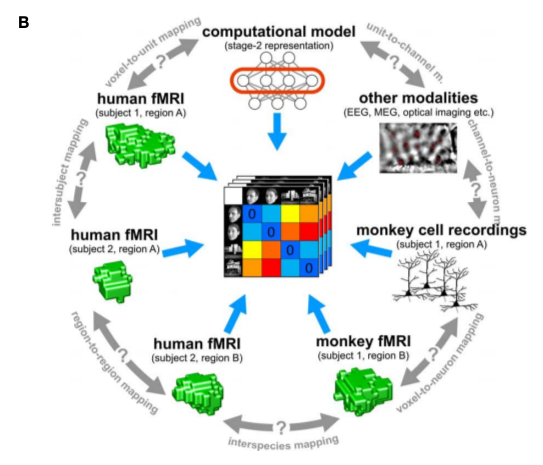
\includegraphics[scale = 0.3]{k08_b.png}
\end{center}
\end{frame}

\begin{frame}
\frametitle{A typical RSA experiment}
An experiment which demonstrates which regions of the brain differentiate between faces and objects.
\begin{center}
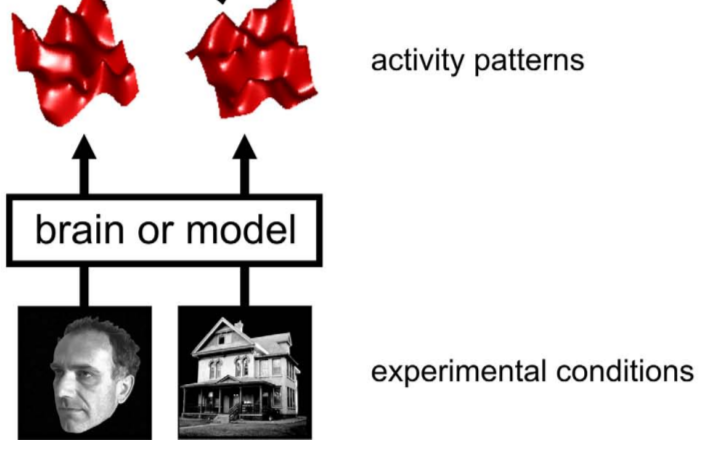
\includegraphics[scale = 0.3]{k08_step1.png}
\end{center}
Step 1: Present the subject with visual stimuli: pictures of faces and houses.
Record the subject's brain activity in the fMRI scanner.
\end{frame}

\begin{frame}
\frametitle{A typical RSA experiment}
Step 2a: Process the data, and represent the brain activity of the subject for the $i$th stimulus as a real vector $y_i$.
Form matrix of distances between $y_i$ and $y_j$, the \emph{representation distance matrix} (RDM)
\begin{center}
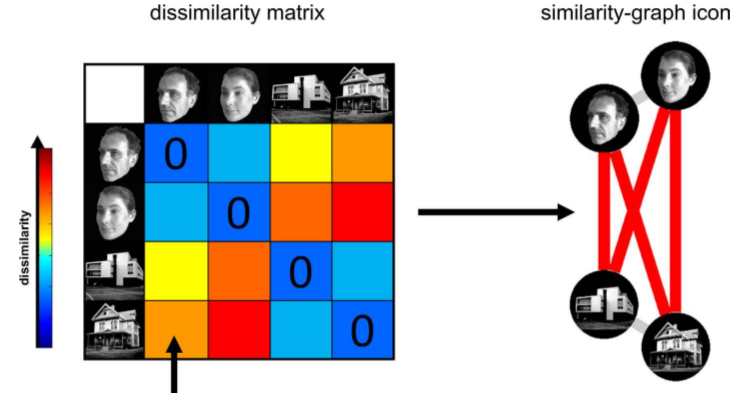
\includegraphics[scale = 0.3]{k08_step2.png}
\end{center}
Step 2b: Assess statistical significance of distances to form similarity graph
\end{frame}

\begin{frame}
\frametitle{A typical RSA experiment}
Step 3: Compare similarity graphs between different brain regions.
\begin{center}
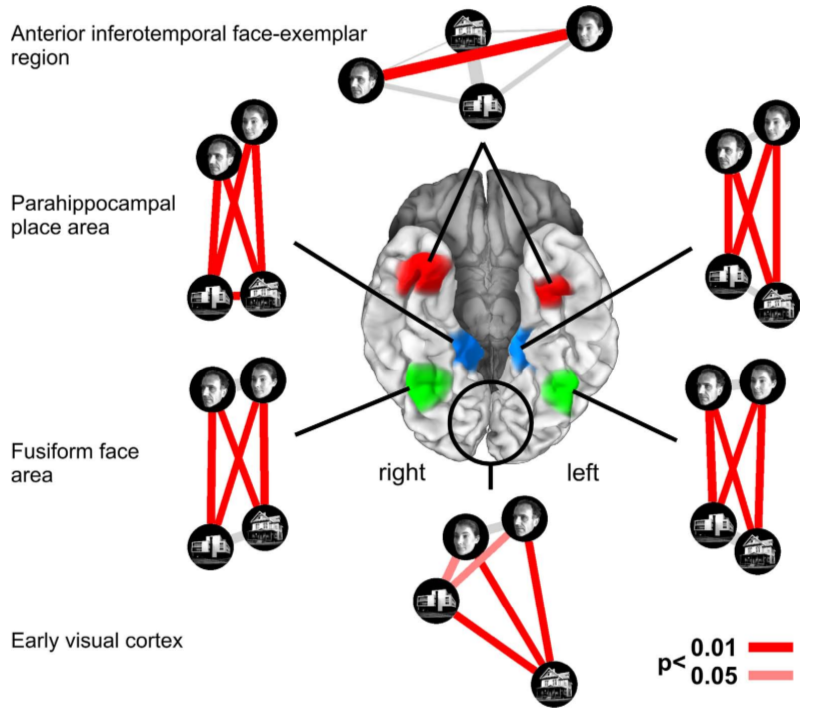
\includegraphics[scale = 0.2]{k08_step3.png}
\end{center}
Step 4: Draw scientific conclusions.  (Step 5: Profit!!..?)
\end{frame}

\begin{frame}
\frametitle{Comparison to parametric approach}
\begin{itemize}
\item RSA is a ``nonparametric'' approach, because stimuli are treated as discrete classes
\item In contrast, one could consider presenting stimuli which are parameterized
\item Example: present the subject with gratings of varying orientation.  Orientation $x$ is parameter
\end{itemize}
\begin{center}
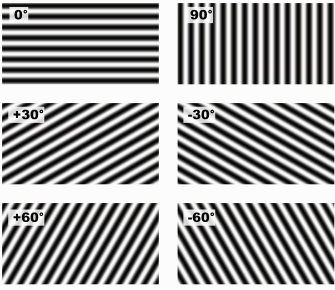
\includegraphics[scale = 0.2]{grating_angle.png}
\end{center}
\end{frame}

\begin{frame}
\frametitle{Example of parametric approach: natural images}
\begin{center}
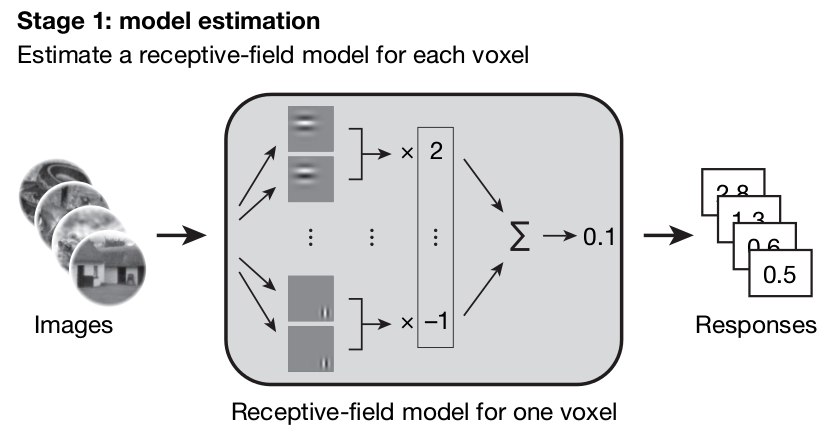
\includegraphics[scale = 0.2]{kay_stage1.png}
\end{center}
\begin{itemize}
\item Kay et al (2008) parameterize natural images using \emph{Gabor filters}
\item Let $x_i$ be the vector of 10000 Gabor filter coefficients for a natural image.
Let $y_i$ be the vector of 20000 individual voxel responses.
\item Kay fits a model of the form
\[
y_i = B^T x_i + \epsilon_i
\]
where $B$ is a 10000 x 20000 coefficient matrix, and $\epsilon_i$ is vector-valued noise with covariance $\Sigma$
\end{itemize}
\end{frame}

\section{Questions}

\section{Proposed Projects}

\end{document}












